\section{Models for signal and background components in invariant mass spectrum}
\label{sec: model}

The expected Signal shape, as well as the expected shape for the combinatorial and physical backgrounds have to be known in order to properly describe the invariant mass distribution of 
$\Bs\to\Ds\kaon\pion\pion$ and $\Bs\to\Ds\pion\pion\pion$ candidates.

\subsection{Signal model}
\label{subsec: signalmodel}
The mass distribution of $\Bs\to\Ds\kaon\pion\pion$ signal is modeled using two gaussian functions, which share the same mean $\mu$, but are allowed to have different widths $\sigma_{1}$ and $\sigma_{2}$. 
Another double gaussian is used to account for the contribution of $\B^{0}\to\Ds\kaon\pion\pion$ decays, which are also present in the $m(\Ds\kaon\pion\pion)$ spectrum. 
All parameters of both double gaussians except the core width $\sigma_{1}$ \comment{Why is it fixed and to what? } are allowed to float in the nominal fit. \newline
The same approach is used to describe the invariant mass distribution of $\Bs\to\Ds\pion\pion\pion$ candidates. 
A double gaussian is used to model this signal shape, all parameters except the core width $\sigma_{1}$ are allowed to float.

\subsection{Background models for $\m(\Ds\pion\pion\pion)$} 
\label{subsec: BkginNorm}
Different background sources arise in the invariant mass spectrum of candidates for the normalization mode. \newline
The following backgrounds have to be accounted for:
\begin{itemize}

\item combinatorial background: This contribution arises from either a real $\Ds$, which is paired with random tracks to form the $\Bs$ candidates, or via real $X_{d}$'s, which are combined with three tracks that fake a $\Ds$ candidate to form a fake $\Bs$.   

\item Partially reconstructed $\Bs\to\Ds^{*}\pion\pion\pion$ decays, with $\Ds^{*}\to\Ds\gamma$ or $\Ds^{*}\to\Ds\piz$, where the $\gamma$/$\piz$ is not reconstructed in the decay chain. 

\end{itemize}

In both cases of combinatorial background, the distribution in the invariant mass spectrum of $\Bs$ candidates is expected to be smooth and decrease with higher masses. 
Therefore, one exponential function is used to model these contributions. \newline
The shape of the  $\Bs\to\Ds^{*}\pion\pion\pion$ contribution is expected to be peaking in the $m(\Ds\pion\pion\pion)$ spectrum, with large tails due to the missing momentum, which is carried away by the $\piz$ or $\gamma$. 
We rely on simulation to estimate the shape of this contribution. 

\begin{figure}[h]
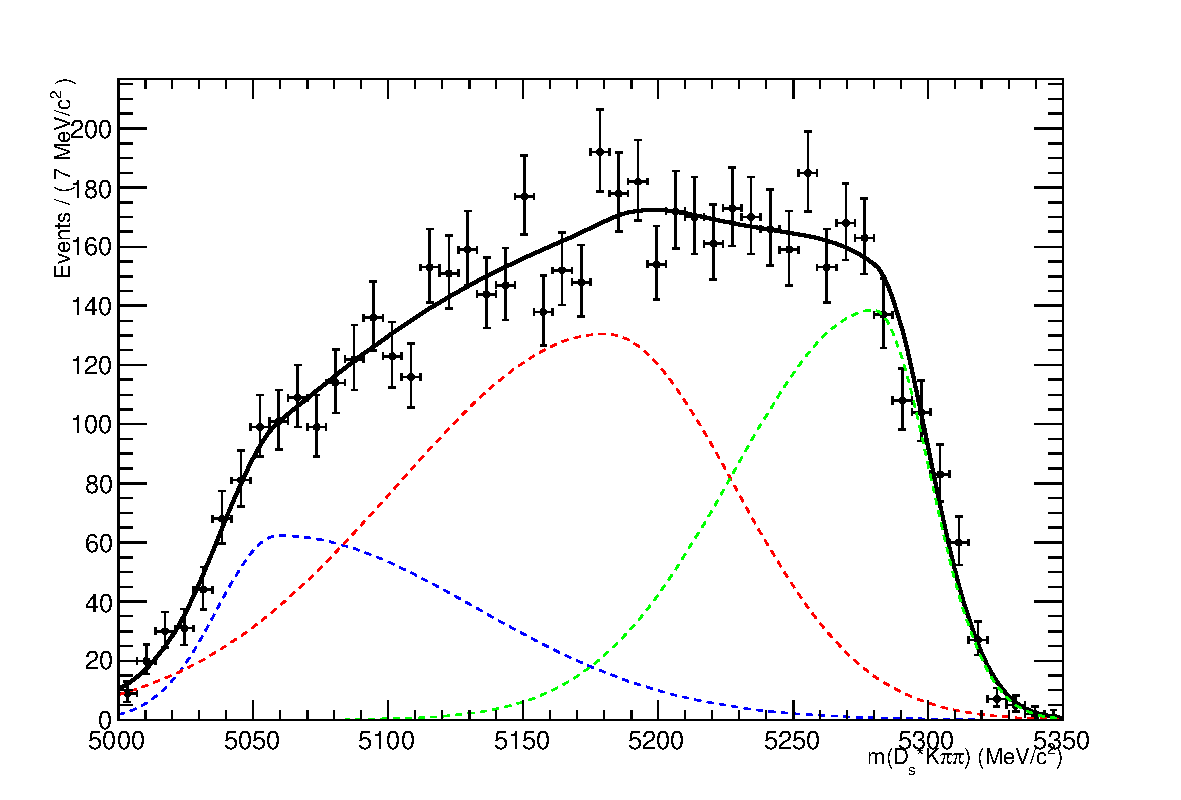
\includegraphics[height=8.cm,width=0.80\textwidth]{figs/Bs2Dsstartpipipi.pdf}
\caption{Invariant mass distribution of simulated $\Bs\to\Ds^{*}\pion\pion\pion$ events, where the $\gamma$/$\piz$ is excluded from the reconstruction. 
A fit of the sum of three bifurcated gaussians to this distribution is overlaid.}
\label{fig: BsDsstar3piMC}
\end{figure}

Figure \ref{fig: BsDsstar3piMC} shows the fit of the sum of three bifurcated gaussians to the invariant mass distribution of simulated $\Bs\to\Ds^{*}\pion\pion\pion$ event. 
The pion or photon from $\Ds^{*}\to\Ds(\gamma/\piz)$ is excluded from the reconstruction. The obtained shape parameters are used as input values for the nominal $m(\Ds\pion\pion\pion)$ mass fit. 
The yield of this contribution is directly determined in the nominal fit. 


\subsection{Background models for $m(\Ds\kaon\pion\pion)$}
For the signal channel, the following background sources have to be considered:

\begin{itemize}

\item combinatorial background: Same contributions as discussed in Sec. \ref{subsec: BkginNorm}.

\item Partially reconstructed $\Bs\to\Ds^{*}\kaon\pion\pion$ decays, with $\Ds^{*}\to\Ds\gamma$ or $\Ds^{*}\to\Ds\piz$, where the $\gamma$/$\piz$ is not reconstructed in the decay chain. 

\item Partially reconstructed $\Bz\to\Ds^{*}\kaon\pion\pion$ decays, with $\Ds^{*}\to\Ds\gamma$ or $\Ds^{*}\to\Ds\piz$, where the $\gamma$/$\piz$ is not reconstructed in the decay chain.

\item miss-identified $\Bs\to\Ds\pion\pion\pion$ decays, where one of the pions is wrongly identified as a kaon $\pion\rightarrow\kaon$.  

\item miss-identified, partially reconstructed $\Bs\to\Ds^{*}\pion\pion\pion$ decays, where one of the pions is wrongly identified as a kaon $\pion\rightarrow\kaon$ and the $\gamma$/$\piz$ from $\Ds^{*}\to\Ds\gamma$/$\piz$ is 
not reconstructed.

\end{itemize}

Again the combinatorial background is expected to be flat in the spectrum of the invariant mass of $\Bs\to\Ds\kaon\pion\pion$ candidates. An exponential function is used to model this contribution.\newline
The shape of the partially reconstructed $\Bs$/$\Bz\to\Ds^{*}\kaon\pion\pion$ background is taken from simulation. 
\comment{I think we take them from the normalization mode}
A MC sample of $\Bs\to\Ds^{*}\kaon\pion\pion$ events, where the $\gamma$/$\piz$ is excluded from the reconstruction, is generated. 
The sum of three bifurcated gaussians is then fitted to the mass distribution of $\Bs$ candidates. The distribution and the overlaid fit is shown in Fig. \ref{fig: BsDsstarKpipiMC}.  

\begin{figure}[h]
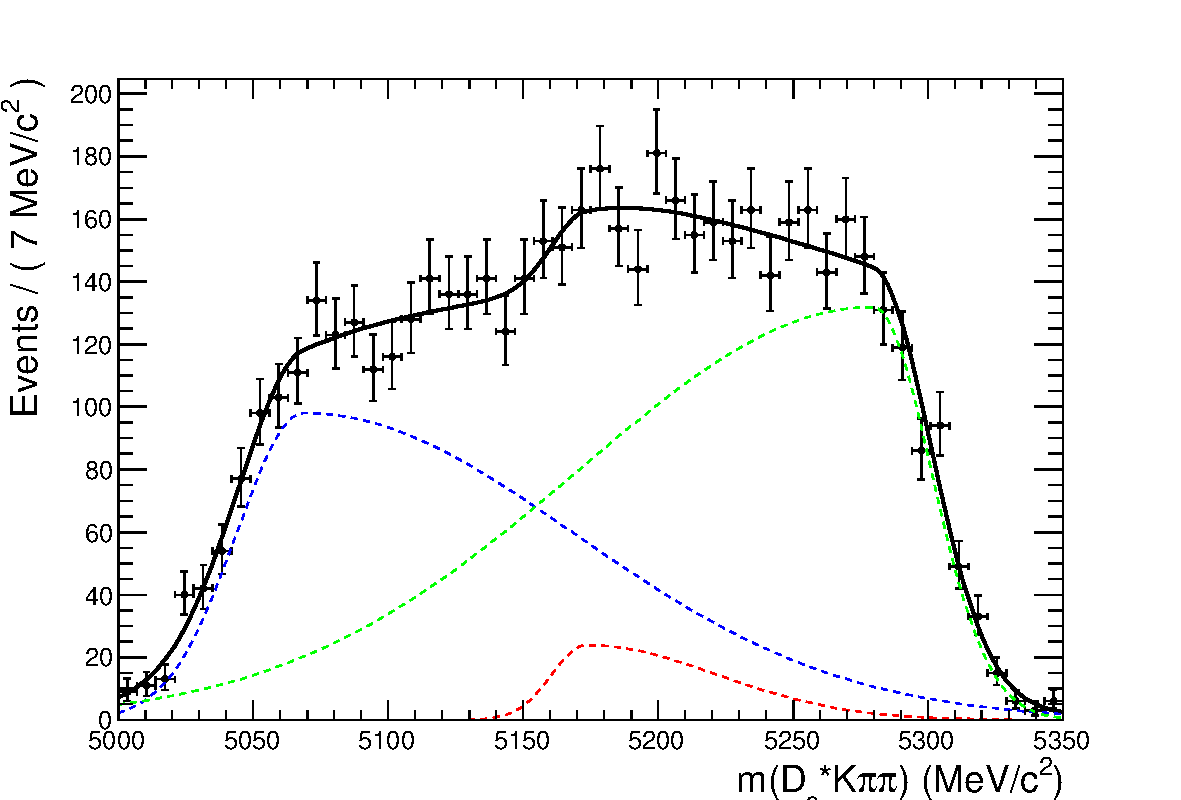
\includegraphics[height=8.cm,width=0.80\textwidth]{figs/Bs2DsstartKpipi.pdf}
\caption{Invariant mass distribution of simulated $\Bs\to\Ds^{*}\kaon\pion\pion$ events, where the $\gamma$/$\piz$ is excluded from the reconstruction. 
A fit of the sum of three bifurcated gaussians to this distribution is overlaid.}
\label{fig: BsDsstarKpipiMC}
\end{figure}

The obtained shape parameters are used as input values for the nominal $m(\Ds\kaon\pion\pion)$ mass fit. For the contribution of the $\Bz\to\Ds^{*}\kaon\pion\pion$ background, the same shape is used, but the means $\mu_{i}$ of the bifurcated gaussians are shifted down by $m_{\Bs} - m_{\Bz}$ \cite{Agashe:2014kda}. The yield of both contributions are directly determined in the nominal fit. \newline
To determine the shape of miss-identified $\Bs\to\Ds\pion\pion\pion$ candidates in the $m(\Ds\kaon\pion\pion)$ spectrum, we take a truth matched signal MC sample of our normalization channel. 
We then use the PIDCalib package to determine the $\pion\rightarrow\kaon$ fake rate. For every candidate in our MC sample, a $p$ and $\eta$-dependent event weight is computed and assigned. 
We flip the particle hypothesis from pion to kaon for the $\pion$ with the biggest miss-ID weight for each event and recompute the invariant $\Bs$ mass. This distribution is then modelled using two crystal ball functions. 
The distribution and fit is shown in Fig. \ref{fig: BsDspipipiMCmissID}(left). 

\begin{figure}[h]
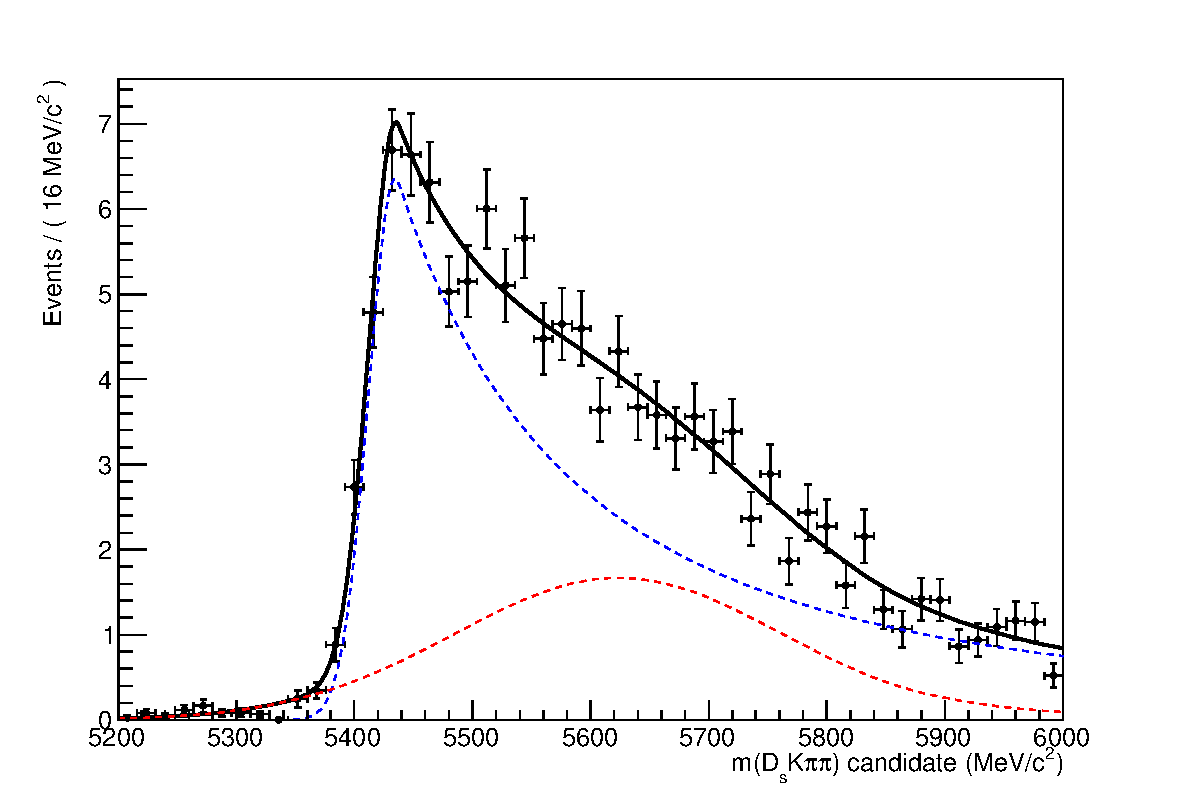
\includegraphics[height=6.cm,width=0.45\textwidth]{figs/Bs2Dspipipi_as_DsKpipi.pdf}
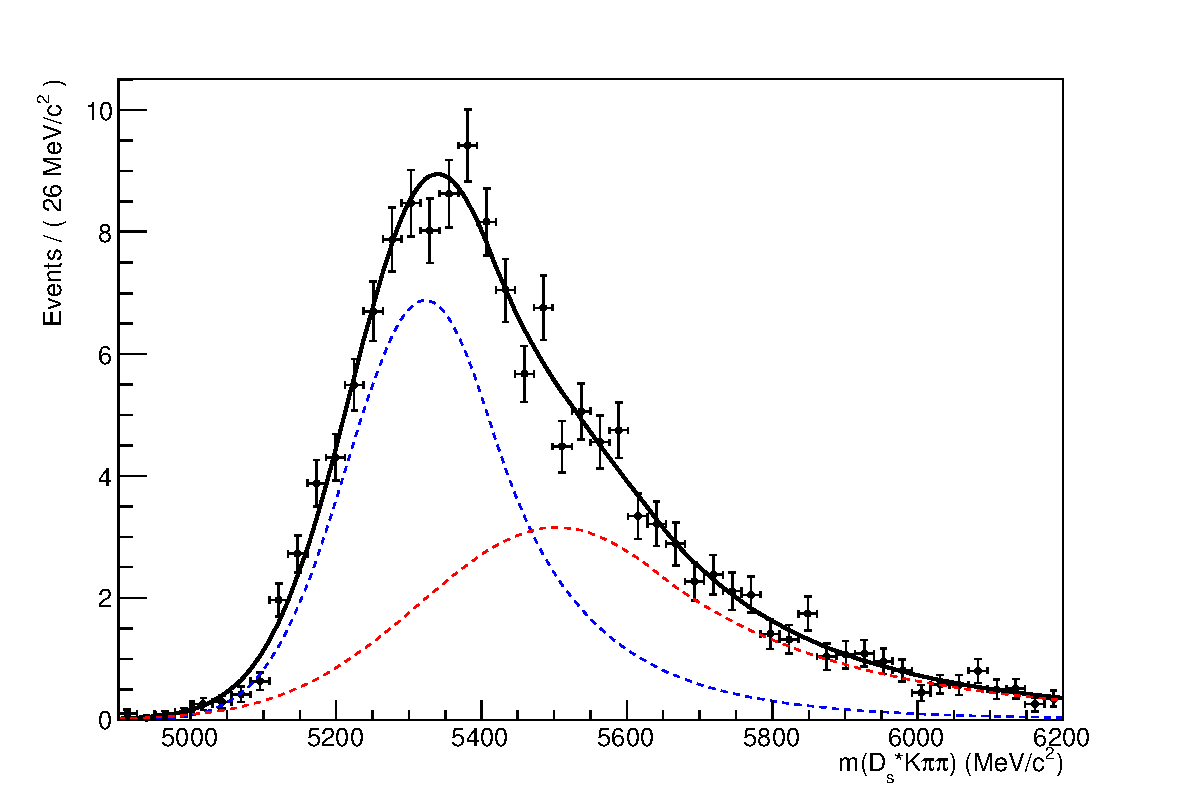
\includegraphics[height=6.cm,width=0.45\textwidth]{figs/Bs2Dsstarpipipi_as_DsKpipi.pdf}
\caption{Invariant mass distribution of (left) simulated $\Bs\to\Ds\pion\pion\pion$ events, where one of the $\pion$'s is reconstructed as a $\kaon$ and the miss-ID probability for each event is taken into account. 
The corresponding distribution for simulated $\Bs\to\Ds^{*}\pion\pion\pion$ events, where the $\gamma$/$\piz$ from the $\Ds^{*}$ is excluded from reconstruction, is shown on the right.
A fit of the sum of two crystal ball functions to each of these distributions is overlaid.}
\label{fig: BsDspipipiMCmissID}
\end{figure}
 
The expected yield of miss-identified $\Bs\to\Ds\pion\pion\pion$ candidates in the $m(\Ds\kaon\pion\pion)$ spectrum is computed by multiplying the fake probability of $\propto3.2\%$, which is derived from PIDCalib, by the yield of $\Bs\to\Ds\pion\pion\pion$ signal candidates, determined in the nominal mass fit of our normalization channel.  \newline
In the same way as mentioned above, we can determine the rate of miss-identified, partially reconstructed $\Bs\to\Ds^{*}\pion\pion\pion$ decays in our sample of $\Bs\to\Ds\kaon\pion\pion$ decays using PIDCalib and a MC sample of $\Bs\to\Ds^{*}\pion\pion\pion$ events. The invariant mass distribution we obtain when we exlude the $\gamma$/$\piz$, flip the the particle hypothesis $\pion\rightarrow\kaon$ and apply the event weights given by the fake rate, is shown in Fig. \ref{fig: BsDspipipiMCmissID} (right). The fit of two crystal ball functions to this distribution is overlaid. 
The yield of this contribution is determined from the yield of $\Bs\to\Ds^{*}\pion\pion\pion$ candidates in the nominal mass fit of our normalization channel, multiplied by the miss-ID probability of $\propto 3.6\%$.

